\chapter{Graphs: traversal and order}\label{ch:graphs}
\index{graph traversal}\index{DFS}\index{BFS}\index{topological sort}

Every graph problem in this book reduces to one question first: what
order do I visit the vertices? Depth-first search dives until stuck
and unrolls the answer on the way back; breadth-first search expands
in layers and thereby measures unweighted distance for free. Built on
them: flood fill for grids, two-colouring for bipartite checks,
Kahn's algorithm for ordering a DAG, and the tail-plus-cycle anatomy
of functional graphs. After this chapter you will choose the
traversal that makes the needed invariant fall out, write the
adjacency-list idiom without thinking, and reconstruct answers ---
paths, components, orders --- from the arrays the search leaves
behind.

\section{Vocabulary}\label{sec:vocab}\index{graph!vocabulary}
A graph $G = (V,E)$ is vertices plus edges: undirected pairs
$\{u,v\}$, or directed arcs $(u,v)$, possibly weighted. Degree counts
incident edges. A \emph{path} revisits nothing; a \emph{cycle}
returns; connected pieces are \emph{components}. Directed graphs get
their own adjectives: a DAG is acyclic; functional graphs have
out-degree exactly 1.

\section{Representations: adjacency lists only}\label{sec:repr}
\index{adjacency list}
The contest representation is \texttt{vector<vector<int>> g(n+1)}:
memory $O(V{+}E)$, iteration $O(\deg v)$. Adjacency \emph{matrices}
cost $O(V^2)$ and are only for dense tiny graphs. Three traps:
self-loops and multi-edges are legal input (your code must not assume
otherwise); CSES vertices are 1-indexed (size the array $n{+}1$); and
undirected edges are added \emph{both} ways.
\begin{figure}[ht]\centering
% fig29-adjlist.tex -- Figure 7.1: the same triangle as a drawing and as adjacency lists.
% fstyle.tex -- shared TikZ styles for the figures of this book (palette from lifeos.sty).
\tikzset{%
  cell/.style={draw=ink, minimum width=7mm, minimum height=6.5mm, inner sep=0pt, font=\footnotesize, fill=white},
  cellh/.style={cell, fill=accentsoft, draw=accent},
  cella/.style={cell, fill=amberbg, draw=amber},
  cellg/.style={cell, fill=goodbg, draw=good},
  cellx/.style={cell, fill=graybg, draw=slate, text=slate},
  vtx/.style={circle, draw=ink, minimum size=6.5mm, inner sep=0pt, font=\footnotesize, fill=white},
  vtxh/.style={vtx, draw=accent, fill=accentsoft},
  vtxa/.style={vtx, draw=amber, fill=amberbg},
  vtxg/.style={vtx, draw=good, fill=goodbg},
  vtxd/.style={vtx, draw=slate, fill=graybg, text=slate},
  lab/.style={font=\footnotesize, text=slate},
  labA/.style={font=\footnotesize, text=accent},
  labM/.style={font=\footnotesize, text=amber},
  idx/.style={font=\tiny, text=slate},
  arr/.style={-{stealth}, thick, ink},
  arrA/.style={-{stealth}, thick, accent},
  arrM/.style={-{stealth}, thick, amber},
  arrG/.style={-{stealth}, thick, good},
  edge/.style={thick, ink},
  edgeA/.style={thick, accent},
  edgeM/.style={thick, amber},
}%
% \cellrow{prefix}{x0}{y}{style}{v0,v1,...}: a row of cells named prefix0, prefix1, ... (pitch 0.75cm)
\providecommand{\cellrow}[5]{\foreach \v [count=\i from 0] in {#5} {\node[#4] (#1\i) at (#2+\i*0.75,#3) {\v};}}%
% \cellidx{prefix}{n}{start}: index labels under cells prefix0 .. prefix(n-1)
\providecommand{\cellidx}[3]{\foreach \i in {0,...,\numexpr#2-1\relax} {\node[idx, below=0pt of #1\i] {\the\numexpr\i+#3\relax};}}%
% \fitfig{<tikzpicture>}: shrink the picture to \linewidth only when it would overflow.
\ifdefined\fitbox\else\newsavebox{\fitbox}\fi%
\providecommand{\fitfig}[1]{\sbox{\fitbox}{#1}\ifdim\wd\fitbox>\linewidth\resizebox{\linewidth}{!}{\usebox{\fitbox}}\else\usebox{\fitbox}\fi}%

\begin{tikzpicture}[font=\footnotesize]
\node[vtx] (v1) at (0,1.5) {1}; \node[vtx] (v2) at (1.8,1.5) {2}; \node[vtx] (v3) at (0.9,0) {3};
\draw[edge] (v1)--(v2) (v2)--(v3) (v1)--(v3);
\node[lab] at (0.9,-0.9) {triangle: 3 edges};
\node[lab, anchor=east] at (4.6,1.5) {};
\foreach \n/\l [count=\k from 0] in {1/{2,3},2/{1,3},3/{1,2}} {
  \node[cellh, minimum width=6mm] (h\n) at (5.4,1.5-\k*0.85) {\n};
  \node[lab, left=1pt of h\n] {};
  \foreach \t [count=\j from 1] in \l
    \node[cell, minimum width=6mm] (e\n\j) at (5.4+\j*1.0,1.5-\k*0.85) {\t};
  \draw[arr] (h\n) -- (e\n1); \draw[arr] (e\n1) -- (e\n2);
}
\node[lab] at (6.5,-1.0) {adjacency lists: each edge stored twice};
\end{tikzpicture}

\caption{The same triangle two ways. Notice the lists store each edge
twice --- that's the price of $O(\deg v)$ iteration.}
\label{fig:adjlist}
\end{figure}

\section{Depth-first search}\label{sec:dfs}
DFS recurses into the first unseen neighbour; the visited set makes
each vertex processed once, so a full pass is $O(V{+}E)$. Free
applications: component counting (one outer call per component),
reachability, cycle detection by back-edge, and --- on grids ---
flood fill.
\begin{lstlisting}[language=C++,caption={\texttt{dfs.h}: the five-line
idiom.},label={lst:dfs}]
\end{lstlisting}
\lstinputlisting{code/dfs.h}
\begin{figure}[ht]\centering
% fig30-dfsstack.tex -- Figure 7.2: DFS recursion stack on the path A - B - D.
% fstyle.tex -- shared TikZ styles for the figures of this book (palette from lifeos.sty).
\tikzset{%
  cell/.style={draw=ink, minimum width=7mm, minimum height=6.5mm, inner sep=0pt, font=\footnotesize, fill=white},
  cellh/.style={cell, fill=accentsoft, draw=accent},
  cella/.style={cell, fill=amberbg, draw=amber},
  cellg/.style={cell, fill=goodbg, draw=good},
  cellx/.style={cell, fill=graybg, draw=slate, text=slate},
  vtx/.style={circle, draw=ink, minimum size=6.5mm, inner sep=0pt, font=\footnotesize, fill=white},
  vtxh/.style={vtx, draw=accent, fill=accentsoft},
  vtxa/.style={vtx, draw=amber, fill=amberbg},
  vtxg/.style={vtx, draw=good, fill=goodbg},
  vtxd/.style={vtx, draw=slate, fill=graybg, text=slate},
  lab/.style={font=\footnotesize, text=slate},
  labA/.style={font=\footnotesize, text=accent},
  labM/.style={font=\footnotesize, text=amber},
  idx/.style={font=\tiny, text=slate},
  arr/.style={-{stealth}, thick, ink},
  arrA/.style={-{stealth}, thick, accent},
  arrM/.style={-{stealth}, thick, amber},
  arrG/.style={-{stealth}, thick, good},
  edge/.style={thick, ink},
  edgeA/.style={thick, accent},
  edgeM/.style={thick, amber},
}%
% \cellrow{prefix}{x0}{y}{style}{v0,v1,...}: a row of cells named prefix0, prefix1, ... (pitch 0.75cm)
\providecommand{\cellrow}[5]{\foreach \v [count=\i from 0] in {#5} {\node[#4] (#1\i) at (#2+\i*0.75,#3) {\v};}}%
% \cellidx{prefix}{n}{start}: index labels under cells prefix0 .. prefix(n-1)
\providecommand{\cellidx}[3]{\foreach \i in {0,...,\numexpr#2-1\relax} {\node[idx, below=0pt of #1\i] {\the\numexpr\i+#3\relax};}}%
% \fitfig{<tikzpicture>}: shrink the picture to \linewidth only when it would overflow.
\ifdefined\fitbox\else\newsavebox{\fitbox}\fi%
\providecommand{\fitfig}[1]{\sbox{\fitbox}{#1}\ifdim\wd\fitbox>\linewidth\resizebox{\linewidth}{!}{\usebox{\fitbox}}\else\usebox{\fitbox}\fi}%

\begin{tikzpicture}[font=\footnotesize]
% frame: x, number of stack entries, current vertex (A/B/D), caption
\newcommand{\fr}[4]{%
  \node[\ifnum#2>0 vtxh\else vtx\fi] (A#4) at (#1,2.4) {A};
  \node[\ifnum#2>1 vtxh\else vtx\fi] (B#4) at (#1+0.9,2.4) {B};
  \node[\ifnum#2>2 vtxh\else vtx\fi] (D#4) at (#1+1.8,2.4) {D};
  \draw[edge] (A#4)--(B#4)--(D#4);
  \foreach \l [count=\k from 0] in {A,B,D} {%
    \ifnum\k<#2 \node[cellh, minimum width=9mm] at (#1+0.9,0.4+\k*0.7) {\l};\fi}
  \draw[slate] (#1+0.35,0) -- (#1+0.35,2.0) -- ++(0,0) (#1+1.45,0) -- (#1+1.45,2.0) (#1+0.35,0) -- (#1+1.45,0);
  \node[lab, align=center, text width=2.6cm] at (#1+0.9,-0.65) {#3};}
\fr{0}{1}{call A: depth 1}{1}
\fr{3.6}{2}{call B: depth 2}{2}
\fr{7.2}{3}{call D: depth 3}{3}
\fr{10.8}{2}{D returns: pop}{4}
\end{tikzpicture}

\caption{The recursion stack growing and unwinding. Notice vertices
\emph{stay} on the stack while their subtree is explored --- that
resident set is what makes back-edge detection work.}
\label{fig:dfsstack}
\end{figure}

\section{Breadth-first search}\label{sec:bfs}
BFS dequeues in arrival order, so vertices surface in nondecreasing
distance: \texttt{dist[]} is the true unweighted shortest path, and
\texttt{parent[]} reconstructs it backwards.
\begin{lstlisting}[language=C++,caption={\texttt{bfs.h}: dist +
parent, the reconstruction pair.},label={lst:bfs}]
\end{lstlisting}
\lstinputlisting{code/bfs.h}
\begin{figure}[ht]\centering
\begin{tikzpicture}[font=\footnotesize]
% F7.3 BFS waves: 4 frames, vertices lit when dequeued.
\begin{scope}
  \node[circle,draw=slate,fill=accentsoft,font=\tiny] at (1.1,1.0) {s};
  \node[circle,draw=slate,font=\tiny] at (0.4,0.2) {};
  \node[circle,draw=slate,font=\tiny] at (1.1,0.2) {};
  \node[circle,draw=slate,font=\tiny] at (1.8,0.2) {};
  \node[font=\tiny] at (1.1,-0.5) {wave 0: \{s\}};
\end{scope}
\begin{scope}[xshift=3.2cm]
  \node[circle,draw=slate,fill=graybg,font=\tiny] at (1.1,1.0) {s};
  \node[circle,draw=slate,fill=accentsoft,font=\tiny] at (0.4,0.2) {};
  \node[circle,draw=slate,fill=accentsoft,font=\tiny] at (1.1,0.2) {};
  \node[circle,draw=slate,fill=accentsoft,font=\tiny] at (1.8,0.2) {};
  \node[font=\tiny] at (1.1,-0.5) {wave 1};
\end{scope}
\begin{scope}[xshift=6.4cm]
  \node[circle,draw=slate,fill=graybg,font=\tiny] at (1.1,1.0) {s};
  \node[circle,draw=slate,fill=graybg,font=\tiny] at (0.4,0.2) {};
  \node[circle,draw=slate,fill=graybg,font=\tiny] at (1.1,0.2) {};
  \node[circle,draw=slate,fill=accentsoft,font=\tiny] at (1.8,0.2) {};
  \node[circle,draw=slate,fill=accentsoft,font=\tiny] at (2.6,0.2) {};
  \node[font=\tiny] at (1.5,-0.5) {wave 2};
\end{scope}
\begin{scope}[xshift=10.2cm]
  \node[circle,draw=slate,fill=graybg,font=\tiny] at (1.1,1.0) {s};
  \node[circle,draw=slate,fill=graybg,font=\tiny] at (0.4,0.2) {};
  \node[circle,draw=slate,fill=graybg,font=\tiny] at (1.1,0.2) {};
  \node[circle,draw=slate,fill=graybg,font=\tiny] at (1.8,0.2) {};
  \node[circle,draw=slate,fill=graybg,font=\tiny] at (2.6,0.2) {};
  \node[font=\tiny] at (1.5,-0.5) {wave 3: done};
\end{scope}
\end{tikzpicture}

\caption{BFS as expanding waves. Notice every vertex in wave $k$ is
exactly distance $k$ --- the queue order \emph{is} the distance
order.}
\label{fig:bfslayers}
\end{figure}
\begin{example}[CSES \emph{Labyrinth}]\label{ex:labyrinth}
Shortest path through a grid with walls; output the path itself.
\par\smallskip
\textbf{Strategy.} ``Shortest'' and ``unweighted'' together name BFS.
The path is recovered by walking \texttt{parent} from the goal ---
search forward, reconstruct backward.
\par\smallskip
\begin{solution}
\lstinputlisting{code/labyrinth.cpp}
Real output (CSES sample):
\begin{lstlisting}[numbers=none]
YES
9
LDDRRRRRU
\end{lstlisting}
\end{solution}
\end{example}

\section{Flood fill}\label{sec:flood}\index{flood fill}
A grid is an implicit graph: cells are vertices, the four directions
are edges. Flood fill counts components --- and uses an
\emph{explicit} stack, because a 1000$\times$1000 room is a million
frames deep.
\begin{lstlisting}[language=C++,caption={\texttt{floodfill.h}:
iterative, 4-direction, marks by rewriting the grid.},label={lst:flood}]
\end{lstlisting}
\lstinputlisting{code/floodfill.h}
\begin{example}[CSES \emph{Counting Rooms}]\label{ex:rooms}
Count floor-connected regions.
\par\smallskip
\textbf{Strategy.} Every unvisited floor cell starts a new room; fill
it completely before moving on. Component counting is the outer loop
--- the fill is just DFS wearing grid clothes.
\par\smallskip
\begin{solution}
\lstinputlisting{code/counting_rooms.cpp}
Real output (CSES sample):
\begin{lstlisting}[numbers=none]
3
\end{lstlisting}
\end{solution}
\end{example}
\begin{figure}[ht]\centering
% fig32-gridgraph.tex -- Figure 7.4: a grid cell as a vertex with four computed neighbours.
% fstyle.tex -- shared TikZ styles for the figures of this book (palette from lifeos.sty).
\tikzset{%
  cell/.style={draw=ink, minimum width=7mm, minimum height=6.5mm, inner sep=0pt, font=\footnotesize, fill=white},
  cellh/.style={cell, fill=accentsoft, draw=accent},
  cella/.style={cell, fill=amberbg, draw=amber},
  cellg/.style={cell, fill=goodbg, draw=good},
  cellx/.style={cell, fill=graybg, draw=slate, text=slate},
  vtx/.style={circle, draw=ink, minimum size=6.5mm, inner sep=0pt, font=\footnotesize, fill=white},
  vtxh/.style={vtx, draw=accent, fill=accentsoft},
  vtxa/.style={vtx, draw=amber, fill=amberbg},
  vtxg/.style={vtx, draw=good, fill=goodbg},
  vtxd/.style={vtx, draw=slate, fill=graybg, text=slate},
  lab/.style={font=\footnotesize, text=slate},
  labA/.style={font=\footnotesize, text=accent},
  labM/.style={font=\footnotesize, text=amber},
  idx/.style={font=\tiny, text=slate},
  arr/.style={-{stealth}, thick, ink},
  arrA/.style={-{stealth}, thick, accent},
  arrM/.style={-{stealth}, thick, amber},
  arrG/.style={-{stealth}, thick, good},
  edge/.style={thick, ink},
  edgeA/.style={thick, accent},
  edgeM/.style={thick, amber},
}%
% \cellrow{prefix}{x0}{y}{style}{v0,v1,...}: a row of cells named prefix0, prefix1, ... (pitch 0.75cm)
\providecommand{\cellrow}[5]{\foreach \v [count=\i from 0] in {#5} {\node[#4] (#1\i) at (#2+\i*0.75,#3) {\v};}}%
% \cellidx{prefix}{n}{start}: index labels under cells prefix0 .. prefix(n-1)
\providecommand{\cellidx}[3]{\foreach \i in {0,...,\numexpr#2-1\relax} {\node[idx, below=0pt of #1\i] {\the\numexpr\i+#3\relax};}}%
% \fitfig{<tikzpicture>}: shrink the picture to \linewidth only when it would overflow.
\ifdefined\fitbox\else\newsavebox{\fitbox}\fi%
\providecommand{\fitfig}[1]{\sbox{\fitbox}{#1}\ifdim\wd\fitbox>\linewidth\resizebox{\linewidth}{!}{\usebox{\fitbox}}\else\usebox{\fitbox}\fi}%

\begin{tikzpicture}[font=\footnotesize, x=1.15cm, y=0.85cm]
\foreach \x in {0,...,4} \foreach \y in {0,...,3} \draw[slate!60, fill=white] (\x,\y) rectangle +(1,1);
\fill[amber!25] (1,1) rectangle +(1,1);
\foreach \x/\y in {1/2,1/0,0/1,2/1} \fill[accentsoft] (\x,\y) rectangle +(1,1);
\foreach \x in {0,...,4} \foreach \y in {0,...,3} \draw[slate!60] (\x,\y) rectangle +(1,1);
\node[font=\scriptsize] at (1.5,1.5) {$(r,c)$};
\node[font=\scriptsize] at (1.5,2.5) {$(r{-}1,c)$}; \node[font=\scriptsize] at (1.5,0.5) {$(r{+}1,c)$};
\node[font=\scriptsize] at (0.5,1.5) {$(r,c{-}1)$}; \node[font=\scriptsize] at (2.5,1.5) {$(r,c{+}1)$};
\node[lab, align=left, anchor=west] at (5.6,2.5) {one floor cell $=$ one vertex};
\node[lab, align=left, anchor=west] at (5.6,1.5) {4 neighbours by the direction\\ arrays \texttt{dr}, \texttt{dc}};
\node[lab, align=left, anchor=west] at (5.6,0.5) {no graph is stored:\\ neighbours are computed};
\end{tikzpicture}

\caption{One cell, four edges. Notice there is no graph object ---
the neighbours are computed, never stored.}
\label{fig:gridgraph}
\end{figure}

\section{Bipartite checks}\label{sec:bip}\index{bipartite}
Colour as you traverse: every neighbour gets the opposite colour, and
the first conflict certifies an odd cycle. If a pass completes, the
colouring itself is the proof.
\begin{example}[CSES \emph{Building Teams}]\label{ex:teams}
Split pupils so friends land on different teams.
\par\smallskip
\textbf{Strategy.} ``Two groups, no inside edges'' is bipartiteness
rephrased; BFS two-colouring either emits the split or meets its own
edge and prints IMPOSSIBLE.
\par\smallskip
\begin{solution}
\lstinputlisting{code/building_teams.cpp}
Real output (CSES sample):
\begin{lstlisting}[numbers=none]
1 2 2 1 2
\end{lstlisting}
\end{solution}
\end{example}

\section{Directed order: Kahn and the DAG}\label{sec:topo}\index{Kahn's algorithm}\index{topological order}
A DAG admits an order where every edge points forward. Kahn's
algorithm: emit in-degree-0 vertices, decrement their out-neighbours,
repeat. If the queue empties with vertices left, they are exactly the
cycle-entangled ones --- the algorithm detects cycles for free.
\begin{lstlisting}[language=C++,caption={\texttt{toposort.h}: Kahn;
short order $=$ cycle.},label={lst:kahn}]
\end{lstlisting}
\lstinputlisting{code/toposort.h}
\begin{example}[CSES \emph{Course Schedule}]\label{ex:course}
Order $n$ courses satisfying prerequisites.
\par\smallskip
\textbf{Strategy.} Prerequisite edges are a DAG exactly when the task
is possible; Kahn emits the order or exposes the cycle.
\par\smallskip
\begin{solution}
\lstinputlisting{code/course_schedule.cpp}
Real output (CSES sample, one valid order):
\begin{lstlisting}[numbers=none]
3 4 1 5 2
\end{lstlisting}
\end{solution}
\end{example}
\begin{figure}[ht]\centering
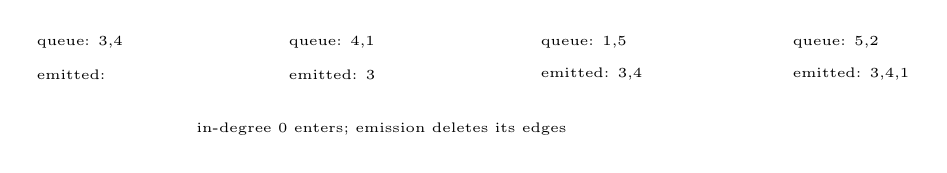
\begin{tikzpicture}[font=\footnotesize]
\foreach \i/\q/\e in {0/{3,4}/{ },1/{4,1}/{3},2/{1,5}/{3,4},3/{5,2}/{3,4,1}}{
  \begin{scope}[xshift=\i*3.2cm]
    \node[font=\tiny,anchor=west] at (0,0.6) {queue: \q};
    \node[font=\tiny,anchor=west] at (0,0.2) {emitted: \e};
  \end{scope}}
\node[font=\tiny] at (4.5,-0.5) {in-degree 0 enters; emission deletes its edges};
\end{tikzpicture}

\caption{Kahn's queue evolution. Notice the emitted sequence is a
\emph{proof}: at print time each vertex's remaining in-degree is 0.}
\label{fig:kahn}
\end{figure}

\section{Functional graphs: tail plus cycle}\label{sec:func}\index{functional graph}
Out-degree 1 means every walk is a tail into a cycle --- the $\rho$
shape of Figure~\ref{fig:rho}. Walks are deterministic, so answers
decompose: distance-to-cycle, then cycle length.
\begin{example}[CSES \emph{Planets Cycles}]\label{ex:planets}
Teleportations until a planet is revisited, per start.
\par\smallskip
\textbf{Strategy.} From any start the trajectory is tail + cycle: the
answer is tail-length + cycle-length. One pass per start, marking as
we go, gives each vertex's answer in $O(n)$ total.
\par\smallskip
\begin{solution}
\lstinputlisting{code/planets_cycles.cpp}
Real output (CSES sample $t=\{2,4,3,1,4\}$):
\begin{lstlisting}[numbers=none]
3 3 1 3 4
\end{lstlisting}
\end{solution}
\end{example}
\begin{figure}[ht]\centering
\begin{tikzpicture}[font=\footnotesize]
\node[circle,draw=slate,font=\tiny] (a) at (0,0) {5};
\node[circle,draw=slate,font=\tiny] (b) at (0.9,0) {4};
\node[circle,draw=slate,fill=accentsoft,font=\tiny] (c) at (1.8,0) {1};
\node[circle,draw=slate,fill=accentsoft,font=\tiny] (d) at (2.7,0.7) {2};
\node[circle,draw=slate,fill=accentsoft,font=\tiny] (e) at (2.7,-0.7) {3};
\draw[-{stealth},slate] (a)--(b) (b)--(c) (c)--(d) (d)--(e) (e)--(c);
\node[font=\tiny] at (0.9,-0.35) {tail};
\node[font=\tiny] at (2.7,1.2) {cycle};
\node[font=\tiny] at (1.4,-1.4) {the $\rho$ shape: every functional
graph is tails feeding cycles};
\end{tikzpicture}

\caption{The $\rho$ anatomy. Notice the tail can be empty --- pure
cycles and self-loops are the same shape with zero stem.}
\label{fig:rho}
\end{figure}

\begin{exercise}[easy]\label{exr:edgecase}
The input may contain a self-loop $(v,v)$ and the parallel edge
$(u,v),(u,v)$. What does each do to your degree counts, BFS layering,
and Kahn's in-degree array?
\end{exercise}
\begin{exercise}[medium]\label{exr:bfsdfs}
On a path graph $1{-}2{-}\cdots{-}n$, state the visit orders of DFS
and BFS from vertex 1. Where do they differ first on a 4-cycle?
\end{exercise}
\begin{exercise}[medium]\label{exr:kahnstop}
Kahn stops early exactly when the leftover subgraph has a directed
cycle. Why can a nonempty acyclic leftover never happen?
\end{exercise}
\begin{exercise}[medium]\label{exr:funcentry}
In a functional graph, show that following successors from any vertex
eventually repeats --- and that the first repeated vertex is always
on the cycle, never mid-tail.
\end{exercise}

\section{Chapter summary}
\begin{table}[ht]\centering
{\small
\begin{tabularx}{\linewidth}{@{}lYYY@{}}
\toprule
\tablehead\thead{Need} & \thead{Tool} & \thead{Cost} & \thead{Leaves behind}\\
\midrule
reach a vertex & DFS & $O(V{+}E)$ & components, order\\
shortest unweighted path & BFS & $O(V{+}E)$ & dist, parent\\
count grid regions & flood fill & $O(nm)$ & painted cells\\
two groups / odd cycle & 2-colour BFS & $O(V{+}E)$ & team array\\
order a DAG & Kahn & $O(V{+}E)$ & topo order or cycle\\
successor structure & walk + stamp & $O(n)$ & tail/cycle split\\
\bottomrule
\end{tabularx}}
\caption{Pick by the invariant you need: layers mean distance, the
stack means depth, the queue's leftovers mean cycles.}
\label{tab:traverse}
\end{table}

\section{Common mistakes}
\index{common mistakes}
\begin{itemize}
\item \textbf{Recursive flood fill on big grids.} $10^6$ cells is a
million-deep call stack --- iterative or explicit-stack only.
\item \textbf{BFS on weighted edges.} Layers are edge \emph{counts};
weights need Dijkstra (Ch~11), and BFS's first visit is no longer
shortest.
\item \textbf{Marking on enqueue vs dequeue.} Mark \texttt{seen} when
\emph{enqueuing}; marking on dequeue lets the same vertex enter the
queue many times --- still correct but quadratic on dense graphs.
\item \textbf{1-indexed off-by-one.} CSES vertices are $1..n$; an
$n$-sized vector drops vertex $n$ silently.
\item \textbf{Forgetting the second direction.} Undirected edges need
two adjacency entries; a one-way insert makes the graph half-directed
and every later claim quietly wrong.
\end{itemize}

\section{Additional exercises}
\begin{exercise}[easy] CSES \emph{Building Roads} --- components + links. \end{exercise}
\begin{exercise}[easy] CSES \emph{Message Route} --- BFS reconstruction. \end{exercise}
\begin{exercise}[easy] USACO-S \emph{Closing the Farm} --- component queries. \end{exercise}
\begin{exercise}[easy] USACO-B \emph{Family Tree} --- ancestor DFS. \end{exercise}
\begin{exercise}[medium] CSES \emph{Round Trip} --- undirected cycle extraction. \end{exercise}
\begin{exercise}[medium] CSES \emph{Game Routes} --- DP on topological order. \end{exercise}
\begin{exercise}[medium] USACO-S \emph{Icy Perimeter} --- flood-fill perimeter. \end{exercise}
\begin{exercise}[medium] USACO-S \emph{Build Gates} --- scaled-cell fill. \end{exercise}
\begin{exercise}[medium] USACO-S \emph{Mooyo Mooyo} --- gravity + fill. \end{exercise}
\begin{exercise}[medium] USACO-S \emph{Visits} --- functional-graph simulation. \end{exercise}
\begin{exercise}[hard] CSES \emph{Monsters} --- multi-source BFS + escape BFS. \end{exercise}
\begin{exercise}[hard] USACO-B \emph{The Great Revegetation} --- signed 2-colouring. \end{exercise}
\begin{exercise}[hard] USACO-S \emph{Snow Boots} --- BFS on (position, boot) state. \end{exercise}

\chapternotes
Traversal order, the adjacency-list idiom and Kahn follow
Laaksonen's graph chapters~\cite{laaksonen2024} and
Sannemo~\cite{sannemo2025}; the USACO Guide's Silver graph modules
carry the same drills~\cite{usacoguide}; the rho-shape framing and
Monsters-style multi-source tricks are in
cp-algorithms~\cite{cpalgorithms} and Halim~\cite{halimcp4}; archive
problems are official CSES/USACO~\cite{cses}.

\section*{Further reading}
\begin{itemize}
\item USACO Guide, ``Graph Traversal'' (intermediate).
\url{https://usaco.guide/silver/graph-traversal} --- BFS/DFS with the
same adjacency-list convention, more problems.
\item USACO Guide, ``Depth First Search'' (intermediate).
\url{https://usaco.guide/silver/dfs} --- the recursive form of
\S\ref{sec:dfs} plus flood-fill on grids.
\item USACO Guide, ``Functional Graphs'' (intermediate).
\url{https://usaco.guide/silver/func-graphs} --- the successor-graph
machinery behind \S\ref{sec:func} (\ref{ex:planets}, \ref{ex:teams}).
\item Laaksonen, \emph{Competitive Programmer's Handbook}, ch.~7
``Graph algorithms'' (beginner). \url{https://cses.fi/book/book.pdf}
--- the whole chapter's vocabulary in forty pages.
\item CSES 1192 \emph{Counting Rooms} and 1193 \emph{Labyrinth}
(practice). \url{https://cses.fi/problemset/task/1192} ---
\ref{ex:rooms} and \ref{ex:labyrinth} verbatim.
\item CSES 1667 \emph{Message Route} and 1679 \emph{Course Schedule}
(practice). \url{https://cses.fi/problemset/task/1667} --- parent
pointers and Kahn's order as live submissions.
\end{itemize}

\begin{rulebox}[Watch instead]
\smallskip\noindent\textbf{Best first.}
``Lecture 13: Breadth-First Search (BFS)'' --- MIT OpenCourseWare,
51 min --- \url{https://www.youtube.com/watch?v=s-CYnVz-uh4}. Levels,
parent pointers, and the unweighted-shortest-path theorem behind
\S\ref{sec:bfs}; OCW draws layers as ``level sets'', same idea as the
book's frontier.
\smallskip\noindent
``Lecture 14: Depth-First Search (DFS), Topological Sort'' --- MIT
OpenCourseWare, 51 min ---
\url{https://www.youtube.com/watch?v=AfSk24UTFS8}. Edge classification
and the reverse-finish topological order of \S\ref{sec:topo} (the book
shows Kahn's algorithm --- both orders are correct; the lecture's is
DFS-based). Access date 2026-10-10.
\end{rulebox}
